\chapter{定量脑电中电势影响因素:参考模态与电极配置}
\section{引言}
人类脑电图因为无创性、超高的时间分辨率广泛应用在认知神经科学和临床研究中。然而,用电极测量的脑电电位对隐藏在头皮下面的神经活动的代表性而言还是一个争论中的问题。本章旨在系统性地调查参考模态和电极配置如何影响脑电电位的准确性。首先,用神经源空间中的单个偶极子源,通过正演计算我们就可以得到标准的脑电电位,这里又分为11种电极数目的情况(10, 16, 21, 32, 64, 85, 96, 128, 129, 257, 335)。 本章中,通过正演理论计算得到的电位的参考是理想的无穷远参考,这是由正演理论内在决定的。 随后,标准的脑电电位被转换到具有不同参考的记录,包括五种单极参考 (左耳垂, Fz, Pz, Oz, Cz)和三种重参考(连接乳突 (LM), 平均参考 (AR) 和参考电极标准化技术(REST))。 最后,标准脑电电位和转换的脑电记录之间的相对误差关于多种因素进行比较,这些因素包括电极数目、头表电极位置区域、电极分布、偶极子源位置方向以及电极测量噪声和头模型。 本章主要发现,单极参考通常带来较大的电位失真,因此一种在线单极参考记录之后的重参考技术一般需要用来降低这种失真效应。在上面提到的三种重参考中,REST总体上对各种比较的因素比AR有更好的效果,连接耳(LM)表现最差,以及REST对头模型的扰动不敏感。AR的效果受到电极分布以及偶极子方向的制约但与电极数目并无紧密的联系。这些结构表明REST可作为脑电重参考的首选,AR可能作为具有较大电极测量噪声时候的替代选择。我们的发现可能为认知神经科学家和临床医生获得更加准确的脑电电位提供了帮助性建议。

\section{研究背景}
自从1929年人类脑电的发现,头表脑电因为其敏感性、无创性、高时间分辨率等优点已成为大脑研究不可或缺的工具。认知科学家、临床医生、工程师们正在使用脑电分别讲述在认知心理学,神经病精神疾病学以及虚拟现实脑机接口等领域成功应用脑电的故事。脑电的成功应用通常依赖于信号处理方法,包括对时域信号的时频分析\citing{koenig_t_topographic_2001},头皮表面的地形图分析\citing{lehmann_d_multichannel_1971,lehmann_d_eeg_2009},以及大脑源空间的层析成像分析\citing{rd_pascual-marqui_review_1999,grech_r_review_2008,valdes_p_frequency_1992}。这些分析要求对源模型\citing{scherg_m_fundamentals_1990}、头模型、容积传导模型的准确估计或模拟,但最重要的是更加接近准确的脑电电势记录。

为了获得准确的头表记录,我们不仅需要控制各种各样的环境噪声也需要减少非中立零参考的失真效应。原则上,脑电电势是活跃电极与参考电极\citing{nunez_p_l_eeg_1997}之间的电势差。在过去的几十年间,人们一直在追求一种接近的零参考电极,以至于活跃电极能够局部记录到时变电势。然而,在身体表面找到一种不活动或者中立的位点是不可能的。参考的选择还没有得到较好地解决,形成了不一致的用法和无休止的讨论,这就是所谓的“参考电极问题”。 目前,多种多样的参考模态已经提出,包括在线记录参考(常用的各种单点参考),和几种离线重参考如连接耳参考(LM)\citing{garneski_t_m_and_steelman_h_f_equalizing_1958},平均参考(AR)\citing{offner_eeg_1950},和参考电极标准化技术(REST)\citing{yao_method_2001}。以前的研究表明参考的选择对脑电波形和功率谱有重大影响\citing{zhai_y_and_yao_d_study_2004,rellecke_j_emotion_2013,chella_f_non-linear_2017},然后参考的效果受到各种因素特别是电极数目的影响\citing{yao_method_2001,liu_q_estimating_2015,lei_x_and_liao_k_understanding_2017,chella_impact_2016}。

在当前的实际应用中,电极数目参差不齐变动范围很大:如临床中常用10导联或者16导联,认知神经科学研究中常采用64-256导联的高密度阵列,甚至在一些研究中用到多于300导联的超高维阵列\citing{oostenveld_r_and_praamstra_p_five_2001,jurcak_v_1020_2007}。然而,以前对于电极导联数对于重参考效果的的研究局限于21-256导联。现在,我们绝地有必要进行覆盖从10导联到300导联以上的对电极数目进行综合的评价研究。此外,随着电极数目增多,这些电极是怎样分布在头表的呢? 典型地具有21电极数目的国际10-20标准放置系统是标准化电极分布的第一份建议\citing{jasper_h_h_ten_1958}。 然后,10-10和10-5系统是10-20系统的衍生,只是采用了更多的电极并加以命名以满足先进的源成像技术的需要\citing{oostenveld_r_and_praamstra_p_five_2001,jurcak_v_1020_2007,nuwer_m_r_ifcn_1998,chatrian_g_e_and_lettich_e_n_p_ten_1985}。 也就是说,这些系统在原来10-20系统的电极基础上按照相对头表面基于的位置准则定义了更多的电极位置。在本研究中,这一系列系统被成为“10-x”系统。相反,另外一种电极分布由Electrical Geodesics, Inc. (USA) 提出,致力于进行高密度脑电神经成像\citing{michel_c_m_and_lantz_g_getting_2004} 思路是按照测地传感网络(GSN)放置更多的电极,好似是在球面上剖分多边形并指定多边形的中心作为电极位置\citing{tucker_d_m_spatial_1993}。 这里,这种电极分布系统被成为“GSN”分布。这两种电极分布的主要差别在于电极是否也覆盖到面颊和颈部。 在不同的电极分布下,重参考技术矫正电位失真的效果是怎样呢?这个问题过去一直被不自觉地忽视。

本章中我们同时研究了参考模态和电机配置(包括电极导联数目和电极分布)两个主要因素。 最初,我们用各种电极配置通过正演计算仿真生成具有无穷远参考的标准脑电电位。 接下来,标准的无穷远参考下的脑电电位被变换为单点参考记录以及三种典型的重参考(LM,AR 和 REST)。 随后, 无穷远参考下的正演出的电位与其他参考下的相对误差计算出来,显然,这种误差取决于 电极数目和电极分布等因素。

\section{仿真方法}
\begin{figure}[h!]
	\centering
	\includegraphics[width=0.6\textwidth,natwidth=610,natheight=642]{pic/JNE/2.1.pdf}
	\caption{标准脑电电位生成,参考转换,相对误差定义的流程图。给定头模型和电极配置,无穷远参考电位正演生成作为基标准, 标准电位再被转换为不同参考的其他记录。最后,转换参考下的电位与基准电位的相对误差关于参考模态、电极配置和一些其他因素交叉比较。}
	\label{2.1}
\end{figure}
仿真和分析流程如图\ref{2.1}。 简单地说,我们首先构造了2个三层头模型,分别是同心球和真实头形状。 偶极子源假设分布在皮层表面以及大脑三维容积栅格中。然后,一定量的电极按照“10-x”或者“GSN”分布匹配偶何在大脑头皮表面。 再者, 通过正演公式基于无穷远参考的标准电位被仿真得出并进一步转换为5种单点参考记录 (如 左耳(LE)/Fz/Cz/Pz/Oz) 和3种重参考技术 (LM/AR/REST)。最后,最后的参考模态和电机配置就是具有离标准电位最小相对电位偏差的一个。

具体地,三层头模型包括大脑皮层、颅骨、头皮,其相对容积传导率分别为1,0.0125,1。对于同心球头形状 \citing{yao_method_2001,yao_d_high-resolution_2000},对于头表面、颅骨内外表面的半径分别是1.0,0.92,0.87。 源空间由2600个离散偶极子均匀径向垂直分布于大脑皮层(半径=0.86)和1269 * 3正交偶极子均匀分布在皮层下区域的3维栅格中(r ⩽ 0.84)。 一共,同心球面头模型的偶极子数达到6407。另外,真是头模型基于MNI结构像模板ICBM152建立\citing{fonov_v_unbiased_2009,fonov_v_unbiased_2011}。在匹配头表电极之后,我们用边界元法\citing{kybic_j_common_2005}通过正演计算头表电位,用到工具包OpenMEEG\citing{gramfort_a_forward_2011}和 Brainstorm\citing{tadel_f_brainstorm_2011,symond_m_p_gamma_2005}。 三层表面(头表面、颅骨内外)每层由1922顶点组成,颅骨厚度设为4mm。源空间由放在所有皮层端点上的15002 * 3 正交偶极子组成。因此,真实头模型中共考虑45 006个偶极子

\subsection{标准脑电电位生成}
有了头模型和电极坐标,传递矩阵$\mathbf{K}$就可以计算出,大小为电极数$N_e$乘以偶极子源的个数$N_s$。给定单个时刻点所有偶极子源活动的强度$\mathbf{x}$,所有电极上的脑电电位可以通过如下公式得到
\begin{equation}\label{eq2.1}
\mathbf{v}_{\infty}=\mathbf{Kx}
\end{equation}
这里注意到传递矩阵$\mathbf{K}$是基于无穷远参考(IR)\citing{de_munck_j_c_potential_1988,wolters_c_h_efficient_2004}。即,源活动和多通道电位之间的关联协同是基于无穷远处的中立零参考。这里,脑电生产模型是所有偶极子源活动在单个时刻点的线性结合。因此,脑电电位在给定头模型和电极配置下完全由相同时刻点下的源活动决定。因为参考问题是由于偶极子源活动到达活跃电极和参考点,就有必要考虑时间过程。 在本章中,我们仅考虑单个时刻点。 接下来,所有偶极子源依次检测以减小由于主观选择源位置的偏差效应。所以,总体上$N_e$乘以$N_s$个标准脑电电位生成以进行误差估计。 确切地,由于\eqref{eq2.1}的线性,不同源活动的随意结合可以相似地估计评价。
\subsection{传感器电极噪声测试}
实际中,不可避免地会有电极测量噪声混合进入到记录的脑电信号中。我们采用零均值多变量高斯分布生成电极测量噪声$e$,噪声可能产生于各种未知的源。因此,脑电生成模型\eqref{eq2.1}变为
\begin{equation}\label{eq2.2}
\tilde{\mathbf{v}_{\infty}}=\mathbf{v}_{\infty}+\mathbf{e},\mathbf{e}\sim{N(\mathbf{0},\mathbf{I}_{N_e})}
SNR=10log_10(lVert\mathbf{v}_{\infty}rVert_2^2\div{\lVert\mathbf{e}\rVert_2^2})
\end{equation}
这里,$\mathbf{0}$是一个$N_e$乘1的零向量,$\mathbf{I}_{N_e}$是$N_e$乘$N_e$的单位矩阵; SNR是干净脑电信号$\mathbf{v}_{\infty}$传感器电极噪声$\mathbf{e}$的能量比例,以分贝为单位;$\lVert·\rVert_2^2$指的是$\ell_2$模的平方。
\subsection{电极放置}
\begin{figure}[h!]
	\centering
	\includegraphics[width=0.6\textwidth,natwidth=610,natheight=642]{pic/JNE/figure2.png}
	\caption{电极配置策略. (a) shows the five mono-polar reference electrodes, that is, LE, Fz, Pz, Oz, Cz and 2 mastoids (Lm, Rm) used for linked mastoids (LM). The table in (b) summarized the channel number (CN) and electre layouts where '10-20 c'—clinically used 10-20 system; '10-20 j'—international 10-20 system standardized by [20]; '10-10 c'—commercially available 10-10 system (Brain Products Co. Ltd, Germany); '10-10 n'—standard 10-10 system extended by [21]; '10-10 r' and '10-05 r'—10-10 and 10-05 system defined by [18]; 'GSN 129/257'—Geodesic Sensor Net polygon placement system innovated by [24]. (c) Shows the details of the electrode layouts.}
	\label{2.2}
\end{figure}
我们研究了11种不同类型的电极数目和2种电极分布,前后二者都可能影响脑电电位的准确性。 电极数目是10, 16, 21, 32, 64, 85, 96, 128, 335通道使用的是“10-x”分布,和129、257通道,使用的是“GSN”电极分布,如图\ref{2.2}所示。 详细地,关于三维电极笛卡尔坐标的的来源,10,16和21 通道的取自10-20电极分布\citing{jasper_h_h_ten_1958};32, 64, 96 和 128 电极 使用的 ‘10-10 c’
分布,取自ActiCHamp 128Ch 标准 (Brain Products Co. Ltd, 德国); 129 和 257 通道取自 the HydroCel™ Geodesic Sensor Net E001 (Electrical Geodesics, Inc., 美国); 64 通道 使用的是 ‘10-10 n’ 分布,85通道用的是 ‘10-10 r’ 分布, 335 通道的坐标是取自
10-05系统\citing{oostenveld_r_and_praamstra_p_five_2001}。
\subsection{参考模态}
一般,所有的参考转换过程可以用公式表示为
\begin{equation}\label{2.3}
\mathbf{v}_r=\mathbf{Tv}_{\infty}
\end{equation}
这里$\mathbf{v}_{\infty}$是无穷远参考下的脑电电位,$\mathbf{T}$指得是特定参考下的转换矩阵。 $\mathbf{v}_r$是转换为参考$r$时的脑电电位。
\subsubsection{在线记录参考}
单极记录参考的原理是从所有活跃电极上减去单极物理参考电极的电位,即,
\begin{equation}\label{2.4}
\mathbf{T}=\mathbf{T}_{r},\mathbf{T}_{r}=\mathbf{I}_{N_{e}}-\mathbf{1f^T},\mathbf{f}=[0,...,1,...,0]^T
\end{equation}
这里$\mathbf{1}$是一个$N_{e}$乘以1的单位向量,$\mathbf{f}$是一个是一个$N_{e}$乘以1的向量但只有一个非零元为1位于单极参考对应的行中,单极参考可能是左侧耳垂LE,Fz,Pz,Oz和Cz。

\subsubsection{重参考技术}
重参考是基于测量的脑电电位的更进一步,在线记录参考过程已经固有的参与当中。

连接耳参考 (LM)
\begin{equation}\label{2.5}
\mathbf{T}=\mathbf{(I-1f^T)T}_{r},\mathbf{f}=[0,...,0.5,...,0.5,...0]^T
\end{equation}
这里$f$是仅具有两个非零元0.5位于左右乳突对应行的零向量。

平均参考 (AR)
\begin{equation}\label{2.6}
\mathbf{T}=\mathbf{(I-1f^T)T}_{r},\mathbf{f}=[1\div{N_e},...,1\div{N_e}]^T
\end{equation}
这里$\mathbf{f}$的所有元是$1\div{N_e}$.

Reference electrode standardization technique (REST)

将等式\eqref{eq2.1}和等式\eqref{2.4}代入\eqref{2.3},我们得到$\mathbf{v}_r=\mathbf{T}_{r}\mathbf{Kx}$。根据等效偶极子源原理\citing{yao_method_2001,yao_d_high-resolution_2000},头表电位$\mathbf{v}_{\infty}$由源$x$通过传递矩阵$K$生成,等效地,也可以通过等效源$x_1$和传递矩阵$K_1$得到,即
\begin{equation}\label{2.7}
\mathbf{v}_{\infty}=\mathbf{Kx}=\mathbf{K}_1\mathbf{x}_1
\end{equation}
这里,$\mathbf{x}_1$可以是分布在二维皮层薄片栅格上覆盖了所有实际偶极子在内的等效源,也可以是与实际的源重叠的三维分布源,或者是在坐标系统远点上的多极源 \citing{yao_d_high-resolution_2000}。 对于REST,尽管正确的源$x$和正确的传递矩阵$K$是未知的,我们可以使用以为的等效源$\mathbf{x}_1$和相应的传递矩阵$\mathbf{K}_1$\citing{yao_method_2001,zhai_y_and_yao_d_study_2004}。在本章中,球面头模型和真实头模型分别用三维栅格上具有三个正交方向的偶极子源和皮层上偶极子具有固定的径向于皮层的方向作为$\mathbf{x}_1$。 因为脑电逆问题是参考无关的\citing{pascual-marqui_r_d_and_lehamann_d_topographic_1993,geselowitz_d_b_zero_1998},$\mathbf{x}_1$的近似估计是
\begin{equation}\label{2.8}
\hat{x}_1=(\mathbf{T}_{r}\mathbf{K}_1)^{+}\mathbf{v}_r
\end{equation}
通过代入公式\eqref{2.8}和\eqref{2.3}代入到\eqref{2.7},无穷远参考下的脑电电位$\mathbf{v}_{\infty}$可以近似地重建为
\begin{equation}\label{2.9}
\mathbf{v}_{rest}=\mathbf{K}_1\hat{\mathbf{x}_1}=\mathbf{K}_1(\mathbf{T}_{r}\mathbf{K}_1)^{+}\mathbf{T}_r\mathbf{v}_{\infty}
\end{equation}
因此,REST的参考转换矩阵是$\mathbf{T}=\mathbf{K}_1(\mathbf{T}_{r}\mathbf{K}_1)^{+}\mathbf{T}_r$。
\subsection{头模型干扰测试}
本质上,REST的效果依赖于头模型的准确度,因为$\mathbf{K}_1$从$\mathbf{K}$变换得到,随着$\mathbf{x}_1$与$x$之间的等效。假设$\mathbf{K}_1$近似于$\mathbf{K}$,我们感兴趣是否REST对头模型的扰动敏感。在以前的研究中,这种扰动是主观改变电极位置\citing{liu_q_estimating_2015}或者通过改变传导率的方式\citing{yao_method_2001,zhai_y_and_yao_d_study_2004}。 这种主观扰动在64通道(‘10-10 c’分布) 上重新检测,我们重新计算$\tilde{\mathbf{K}_1}$ 作为扰动的$\mathbf{K}_1$,用各种各样的结合,这包括两种头形状,11种颅骨传导率和5种源方向,这些在小节\ref{ch3.7}中列出。

为了更加接近实际中的一般情况,$\mathbf{K}_1$是$\mathbf{K}$被给定一个客观的扰动,这种扰动来自于头模型、传导率、电极位置和其他在实际中难以定量描述的未知因素。把等式$\eqref{eq2.2}$和等式$\eqref{2.9}$
放在一起,就成为
\begin{equation*}
\mathbf{v}_{\infty}=\mathbf{Kx}
\mathbf{v}_{rest}=\mathbf{K}_1(\mathbf{T}_r\mathbf{K}_1)^{+}\mathbf{T}_{r}\mathbf{v}_{\infty}
\end{equation*}
理想情况下,$\mathbf{K}$和$\mathbf{K}_1$都应该用精确的头模型和电极分布计算得到。这里,$\mathbf{K}$是用精确的头模型和真正的源活动计算得到,$\mathbf{K}_1$使用扰动的头模型和假设的等效源计算得到。为了增加扰动误差,零均值多变量高斯噪声$\mathbf{e}_1^j$注入到传递矩阵向量$\mathbf{k}_1^j$对应于$\mathbf{k}_1$的$j^{th}(j=1,...,N_s)$偶极子源,即为
\begin{equation*}
\tilde{\mathbf{k}_1^j}=\mathbf{k}_1^j+\mathbf{e}_1^j,\mathbf{e}_1^j\sim{N(\mathbf{0},\mathbf{I}_{N_e})}
SNR_1=10log_10(\lVert\mathbf{k}_1^{j}\rVert_2^2\div{\lVert\mathbf{e}_1^{j}\rVert_2^2})
\end{equation*}
这里$SNR_1$指的是$\mathbf{k}_1^j$对噪声能量的比例,单位为分贝dB。

相应地,REST的重建模型就转换为
\begin{equation}\label{2.9}
\mathbf{v}_{\infty}=\mathbf{kx}
\tilde{\mathbf{v}}_{\infty}=\tilde{\mathbf{K}}_{\infty}(\mathbf{T}_{r}\tilde{\mathbf{K}}_{\infty})^{+}\mathbf{T}_{r}\mathbf{v}_{\infty}
\end{equation}
这里,我们变$\mathbf{K}_1$为$\tilde{\mathbf{K}}_1$作为对头模型、传递矩阵的扰动。

\subsection{影响比较}
给定一个头模型,传递矩阵的值随着电极数目和电极分布而变化。通过设置单个偶极子源具有单位强度的活动而其他源强度为零的神经源活动,多通道脑电电位数值上就等于对应于这个偶极子源的传递矩阵向量。因此,脑电电位受到电极配置的影响。为了检查这种效应,考虑所有电极或某个头表局部区域上的电极的相对误差可以作为一种指标。被$j^{th}$个偶极子生成的电位的相对误差的计算如下
\begin{equation*}
re(j)=\sqrt{\sum_{i=1}^n(\mathbf{v}_r(i)-\mathbf{v}_{\infty}(i))^2}\div\sqrt{\sum_{i=1}^n(\mathbf{v}_{\infty}(i))^2}
\end{equation*}
这里$n$是电极数目(等于阵列大小)或者某个局部头皮区域上的电极数目,$\mathbf{v}_{\infty}$某种电极配置下的正演出的脑电电位,$\mathbf{v}_r$具有某种参考的脑电电位。为了避免源位置的偏差,我们计算大量偶极子源群体水平上的平均相对误差,而不是个体水平上每个偶极子的相对误差。在源空间或这感兴趣神经源区域,相对误差(RE)重新定义为
\begin{equation*}
RE=\sum_j=1^{N_d}re(j)\div{N_d}
\end{equation*}
这里$N_d$指的是整个源空间上或者某个感兴趣源区域的偶极子源的个数。 另外,标准偏差(SD)的计算公式是
\begin{equation*}
SD=\sqrt{\sum_j=1^{N_D}(re(j)-RE)^2\div{N_d-1}}
\end{equation*}
以计算关于偶极子源位置的某种因素的鲁棒性。

\section{结果}
比较参考变换前后的相对误差,我们旨在发现采集的脑电电位如何受到感兴趣的因素的影响。在本小节中,首先,所有电极上的相对误差关于所有的参考模态这个因素进行比较;然后,电极数目和电极分布的效果被分析; 再者,我们总结了关于偶极子源位置方向和电极噪声相对误差比较结果;最后,我们描述了使用真实头模型电极数目这一因素的影响。在总结结果之前,我们声明1)两种头模型是按照完全一致的仿真和分析流程进行的;2)由于两种头模型的结果十分相似,图\ref{2.3,2.4,2.6,2.7,2.8} 仅仅是三层同心球面模型的结果, 图\ref{2.5,2.9}  展示了两种头模型关于电极分布和头模型扰动的比较结果。
\begin{figure}[h!]
	\centering
	\includegraphics[width=0.6\textwidth,natwidth=610,natheight=642]{pic/JNE/figure3.png}
	\caption{Potential relative error as to reference montages. To differentiate the two 64-channels, '64c' and '64n' hereafter mean 64 channels with '10-10 c' and '10-10 n' layout, respectively. The color in each square corresponds to the RE (in percentage) in the colorbar. The RE is the mean of potential relative errors by repeated simulation with 6407 dipoles individually activated. The standard deviation (SD) of the relative errors over 6407 dipoles are shown in figure 4, especially for AR and REST. Topographies with the same colorbar show the effects (RE in percentage) of all the reference montages compared with infinity reference (IR).}
	\label{2.3}
\end{figure}
\subsection{参考模态的影响}
图\ref{2.3}具有分级颜色的图像显示了八种参考模态所有电极上电位的相对误差。 不进行重参考,只有单极参考(LE, Fz, Pz, Oz, Cz)相对误差大于61.5\%;通过连接乳突LM重参考之后,相对误差降低到41\%。 特别地,AR和REST的使用使得相对误差降低到大约17\%和2.7\%,显然更加无偏差的电位。 这说明:(1) 重参考是不可或缺的,以矫正单极记录参考的较大的失真效应;(2) REST和AR比LM更具有优势;(3) REST是矫正所有电极上电位所有参考方法中最优的一个。 围绕着中心的一个——无穷远参考的地形图的其他八个地形图展示了257通道电极数目上参考模态的效果比较。 中心的一个展示了五个皮层偶极子生成的标准电位的分布和强度。参考变换之后,八种参考的电位使用与无穷远参考相同的颜色尺度作为比较。显然,相对大的颜色改变在参考为LE, Fz, Pz, Oz, 和 Cz 的地形图上表明在线记录参考对电位的失真效应,然而底下的三种地形图显示了离线重参考的矫正效应。
\subsection{电极数目的影响}
从这一小节开始,我们重点比较REST和AR,因为二者远远领先于其他参考模态。电极数目的效果就稀疏阵列和致密阵列来评价。 在所有电极(AS)相对误差结果上,我们也计算了部分电极上的相对误差。基于地形图拓扑传统,AS被划分为部分电极,分别是额叶电极frontal sensors
(FS),颞叶电极(TS),顶叶电极 (PS) 和枕叶电极 occipital sensors (OS)。 图\ref{2.4}中的二维电极分布显示了我们如何用红线划分64个电极。由于左右颞叶电极的对称性,我们接下来只考虑左侧颞叶。 因为图\ref{2.4}的Y轴
使用以10为底的log尺度,因此明显地AR具有比REST更高的相对误差,不论是在所有电极上还是致密阵列的部分电极上。 在稀疏阵列的部分电极上,REST的相对误差在21和32通道时还比AR小很多;在10和16通道的电极数目下,REST的相对误差较大但还是比AR的相对误差要小。 这说明REST甚至能够在十分稀疏的阵列中取得比AR更好的效果。REST比AR较小的相对误差不仅表现在所有电极上还表现在部分电极上。这表明REST不受电极数目的影响总是在矫正脑电电位上具有比AR更好的效果。
\begin{figure}[h!]
	\centering
	\includegraphics[width=0.6\textwidth,natwidth=610,natheight=642]{pic/JNE/figure4.png}
	\caption{Potential relative error as to channel number. The charts separated by the dash lines show the REs of all arrays (10-335), sparse array (≤32) and dense array (≥64), respectively. The Y axes are displayed in 10-base logarithm scale. The REs and SDs (error bar) are the mean and standard deviation of the relative error of the potentials over all sensors, or a partial sensors region.}
	\label{2.4}
\end{figure}
AR的相对误差没有随着电极数目的增多呈现线性下降的趋势。这意味着致密的电极阵列未能改善AR的性能。也就是说,电极数目或者电极密度对AR来说不是至关重要的。该结果并不和广泛的共识相一致,该共识认为AR的优势仅仅来自于大量的电极数目和头表面电极宽泛覆盖\citing{christodoulakis_m_effect_2013}。
最后,REST的标准偏差总是比AR的标准偏差小。总体来讲,在关于电极数目和头表区域的重复仿真测试中,REST比AR具有更加鲁棒的性能。

\subsection{电极分布的影响}
\begin{figure}[h!]
	\centering
	\includegraphics[width=0.6\textwidth,natwidth=610,natheight=642]{pic/JNE/figure5.png}
	\caption{Potential relative error as to electrodes layout. The RE is shown in 10-base logarithm scale, while the prefix 's' and 'r' in the horizontal axis mean the spherical and realistic head model used in simulation, respectively. The legend on the right shows '10-x' layout with 'BP128', 'EGI129' setups and 'GSN' layout with 'EGI257', 'BP335' setups. Each setup is displayed on the spherical and realistic head surfaces with the yellow dots representing the electrode position.}
	\label{2.5}
\end{figure}
我们需要把更多的注意力放到128到335电极之间,因为它们具有完全不相似的电极分布。 图\ref{2.5}显示了"10-x"电极分布(‘BP128’, ‘BP335’配置)和 ‘GSN’类型分布(‘EGI129’, ‘EGI257’配置)之间的电位相对误差比较。 每种配置配准在球面或者实际头模型表面上,以便于直观地了解每一种配置的分布位置。‘BP128’和‘BP335’分别按照‘10-10 c’和‘10-05’系统,但二者均只有头上表面区域被大量电极均匀覆盖。 相反,除了完全不同的电极放置准则,更多的区域例如下巴和脖子也被‘EGI129’和
‘EGI257’所采样到。 图\ref{2.5}关于四种电极配置的相对误差对‘s REST’分别是0.50\%, 0.14\%, 0.05\%, 0.27\%和对‘s AR’分别是19.56\%, 11.50\%, 5.67\%, 15.65\%。 显然,相对于"10-x"分布,REST和AR在‘GSN’分布下都产生了更低的相对误差。 这说明了宽泛的电极覆盖对REST有提升作用,但主要对AR带了了巨大的提升。 “BP128”与“EGI129”具有几乎一样多的电极数目但是不同的电极分布,AR的相对误差就从19.56\%下降到11.50\%。但是,在‘BP128’基础上增加200多个电极形成了‘BP335’,后者具有十分高的空间采样和致密的覆盖,我们却发现AR的相对误差仅仅显示了从19.56\%到 
15.65\%的略微下降。 然而,‘EGI257’分布下AR的相对误差减少到‘BP335’相对误差的三分之一,但是仅仅前者比后者有大约80(335-257) 个电极去掉。 如果用实际真实头模型(r)取代了三层同心球面头模型(s), 以上的结果不变。 这些比较说明一方面AR效果的关键因素是宽泛的电极覆盖并非更多的电极数目,另一方面REST在较多电极数的情况下具有比AR更加明显的优势。

\subsection{偶极子源位置的影响}
给定电极配置和头模型,脑电电位仍受到偶极子分布位置的影响。我们将2600个皮层偶极子和1269*3正交栅格偶极子按照大脑体素的传统划分分为四个脑区。 
图\ref{2.6}的半个球面显示了图\ref{2.5}中的所有偶极子源是怎样被划分为额叶偶极子 (FD),颞叶偶极子 (TD),顶叶偶极子(PD) 和 枕叶偶极子(OD)。 图\ref{2.6}的柱状图显示了所有电极电位的相对误差但是区别在于分别是由单个感兴趣的脑区生成的。 FD, TD, PD 
和 OD生成的脑电电位的相对误差分别是顺次从左顶端到右下端柱状图中画出。REST和AR的相对误差分别是显示为蓝色和黄色。 总体上,不论偶极子源分布于哪个脑区,REST总能产生比AR更小的相对误差。
\begin{figure}[h!]
	\centering
	\includegraphics[width=0.6\textwidth,natwidth=610,natheight=642]{pic/JNE/figure6.png}
	\caption{Potential relative error as to dipole source position. The semi-sphere shows the coordinates system and the source space of 3-layer concentric spherical head model. XYZ axes are oriented from the origin to the nasion, towards to the left ear, and directed to the vertex, separately. RE and SD (error bar) are the mean and standard deviation of the potential relative error over all sensors with partial dipoles in one source region individually activated, respectively.}
	\label{2.6}
\end{figure}

\subsection{偶极子源方向的影响}
除了源活动的位置,源活动的方向也可能对获取的脑电电位准确率有较大的影响。图\ref{2.7}显示了靠近皮层径向活动的偶极子或者一个体素栅格偶极子沿着XYZ三个正交方向中的其中一个活动所产生的脑电电位的相对误差。 REST和AR之间的相对误差在X和Y方向上并没有表现出像Z方向上的相当大的差异,但是REST和AR在Y方向上比在X方向上表现出更明显的相似性。对于靠近皮层的径向偶极子,REST和AR相对误差的差异程度似乎是XYZ三个方向上差异的折中。该结果可能和电极位置的空间对称性的程度有关。 我们再次注意到图\ref{2.2}
中如果把二维电极分布转换到球面或者实际头模型如图\ref{2.5}的三维电极分布,我们发现左右电极区域完美的对称性,前后电极区域很好但是不很完美的对称性,上下电极区域特别差的对称性。另外,关于偶极子源各个方向的上相似的相对误差表明了REST能够鲁棒地矫正脑电电位。AR在径向和Z反向上比XY方向上大得多的相对误差可能警示我们AR受到偶极子源活动方向的制约但可能只适合于对于水平横断面上活动的偶极子。
\begin{figure}[h!]
	\centering
	\includegraphics[width=0.6\textwidth,natwidth=610,natheight=642]{pic/JNE/figure7.png}
	\caption{Potential relative error as to source orientation. 3D plot displays the radial orientation of cortical dipoles in blue diamonds and XYZ three orthogonal directions of grid dipoles in red diamonds, respectively. RE and SD (error bar) are the mean and the standard deviation of potential relative error over all sensors with cortical dipoles or grid dipoles individually activated.}
	\label{2.7}
\end{figure}

\subsection{传感器电极噪声的影响}
图\ref{2.8}显示了REST和AR对于传感器电极噪声敏感性的比较。 没有电极噪声的情况对应于$SNR=Inf dB$。 从砖红色到蓝色,SNR依次分别是40, 30, 20, 10, 8, 4 和 2 dB。 具有相同颜色的标号相互连起来以标绘出随着电极数目变化相对误差的波动趋势。显然,图\ref{2.8}(a) 中虚线的间隔比图\ref{2.8}(b)的大,图\ref{2.8}(a)中的虚线比图\ref{2.8}(b)中的低,除了当257通道具有的宽泛电极覆盖且SNR < 20 dB和SNR ⩽ 4 dB时,AR表现出了在某些电极数目时比REST好那么一点点,分别是21, 64, 96和257。 这些结果表面 (1) REST
可能比AR对传感器电极噪声具有更大的敏感性; (2) 如果脑电混合有很小的噪声时,REST还比AR具有优势,应该会优选 (3) 由于通过简单的平均起到的去噪效应,AR也可能适用于更高噪声的情形。
\begin{figure}[h!]
	\centering
	\includegraphics[width=0.6\textwidth,natwidth=610,natheight=642]{pic/JNE/figure8.png}
	\caption{Potential relative error as to sensor noise. RE is the mean of potential relative error over all sensors with all dipole sources individually activated. (a) the effect of REST; (b) the effect of AR.}
	\label{2.8}
\end{figure}

\subsection{头模型的影响}
\label{ch3.7}
图\ref{2.9}(a) 显示了三层同心球面模型(s)和ICBM152实际头模型(r)。对于这两种头模型,我们采用相同的仿真和分析流程。 REST和AR基于这两种头模型生成的脑电电位相对误差比较对比如图\ref{2.9}(b)所示。红色紫色虚线之间大的间隙证明对于所有电极数目的情况,‘r REST’依然能够获得比‘r AR’低得多的相对误差。
这表明REST的合理性可能不取决于头形状的复杂程度。 为了检查是否REST依赖于头形状的准确程度,颅骨传导率和源空间配置情况,当这三个因素的正确值对于接受脑电记录的被试来说均未知的情况下,无穷远参考下的脑电电位通过使用真实头形状,颅骨相对于大脑传导率设置为0.0125,源配置如图\ref{2.9}(c)的黑色横条中的(1)所示,但是使用REST重建脑电电位时候用的是各种各样因素的组合,例如头形状可能是球形或者真实的(‘s’, ‘r’), 颅骨对大脑传导率设置为(0.0001, 0.0005, 0.0016, 0.0032, 0.0063, 0.0125, 0.025, 0.05, 0.1, 0.5, 1),源空间配置如图\ref{2.9}c中的(2)–(6)所示。 显然,REST比AR的优越性可以在简单的球面头形状,颅骨对大脑传导率为0.0001,源空间配置为 (2)–(6)中十分不同情况都能得到保持。 我们观察到合理的结果:REST的相对误差随着仿真中对头形状、颅骨脑相对传导率,源空间配置的更好近似而减小。为了模拟不精确头模型更一般的情形,我们通过注入噪声检查了“r REST”受到头模型扰动的影响,结果如图\ref{2.9}(d)中所示。 显然,尽管有两倍(-3dB)的噪声注入到REST用的传递矩阵$\mathbf{K}_1$,‘r
REST’仍能够比‘r AR’有更小的误差。 总之,这些结果可能表明REST对头模型的扰动不敏感,在使用不精确的头模型时还可以保持其优势。
\begin{figure}[h!]
	\centering
	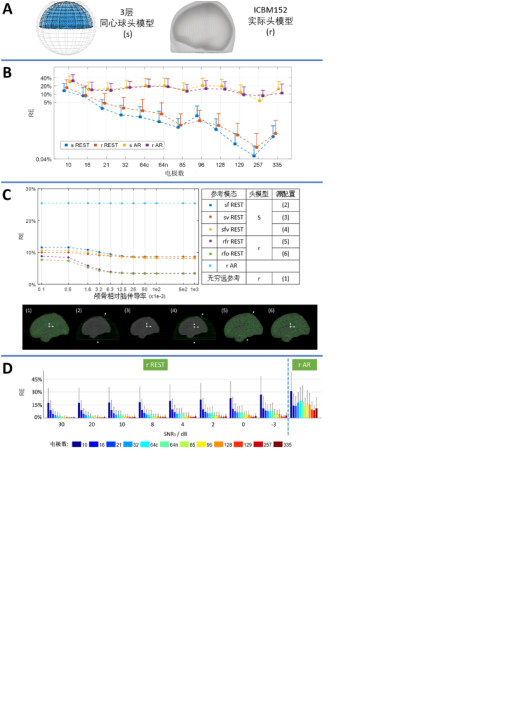
\includegraphics[width=0.6\textwidth,natwidth=610,natheight=642]{pic/JNE/figure9.png}
	\caption{Potential relative error as to head model. (a) The two head models. (b) The REs of potentials generated by the two head models. (c) The effects of perturbated 'r REST' on '64 c' electrodes setup by using different skull conductivities, head shapes, source configuration; the black bar shows 6 source configurations where white arrows display the orientations of dipole source: (1) 17 volume layers and 15 765 * 3 orthogonal dipoles (2) equivalent distributed source layer with 2600 radial cortical dipoles and 400 dipoles perpendicularly to the transverse plane, (3) 1269 * 3 orthogonal volume dipoles, (4) the combination of (2) and (3), (5) 15 002 radial cortical dipoles, and (6) 15 002 * 3 orthogonal cortical dipoles. The prefix of REST in the table, 's, r' means head shape; 'f, v, fv' means 'cortical surface dipoles', 'volume dipoles', and 'surface and volume dipoles', separately; 'r, o' as the third letter denotes radial and orthogonal orientation, respectively. (d) the results of perturbated 'r REST' by injecting noise to the lead field.}
	\label{2.9}
\end{figure}

\section{讨论}
以前的研究已经意识到以标准化脑电记录中立参考估计和电极分布的重要性。例如,脑电数据的获取中双极、单极、平均参考的方法之间相互比较\citing{osselton_j_w_acquisition_1965}, 这最早可以追溯到1965年; Yao提出了REST以近似获取无穷远参考\citing{yao_method_2001}; Quanying
发现高密度阵列对AR是重要的,实际的头模型对REST是至关重要的\citing{liu_q_estimating_2015}; 10-20, 10-10和 10-5 系统 是考虑到相对头表面基于的电极位置系统的合理性相继拓展得到的\citing{jurcak_v_1020_2007}。 然而,还没有研究同时考察了多种可选的参考模态和各种各样的电极配置。 在本章中,我们全面探究了测量的头表脑电电位在哪种程度上受到参考模态、电极分布、电极数目、头皮电极区域、电极分布、偶极子源位置和方向以及电极测量噪声和头模型。

我们发现重参考技术需要应用以矫正使用单极记录参考脑电电位的高度失真,REST可能是一种比广泛使用的AR更好更有潜力的参考。对于电极数目,REST 显示了比AR好得很多的性能,不仅对全部的电极而且对部分头表区域的电极也是这样。 一个惊人的结果AR的效果不随着更多的电极数目得到改善,更加宽泛的电极覆盖对AR是至关重要的。 该结果并非和以前的结果一致,以前的结果显示高密度阵列下AR的使用还可能作为金标准\citing{kayser_j_and_tenke_c_e_search_2010,srinivasan_r_spatial_1998}。另外,无论偶极子源的位置在哪里,REST都能够产生比AR更小的误差。 另外,我们发现AR可能仅对横断面上朝向的偶极子源适合,但REST不论偶极子源的是如何朝向其效果都比较稳定。再者,REST相对AR对电极测量噪声有些敏感,但总体上对一般的情况都具有更好的效果。最后,对真是头模型进行扰动并重复分析测试显示REST的优势甚至在不太精确的头模型时也依然保持。

这些结果可能表明REST能够鲁棒地重建脑电电位,但是AR受到电极覆盖区域和偶极子源方向的制约。二者的鲜明差异可以从它们物理学上的理论假设得到解释。
AR的物理假设是容积导体上的电位表面积分为零
\citing{schiff_s_j_dangerous_2005,bertrand_theoretical_1985,nunez_p_l_and_srinivasan_r_notitle_2006}。
新的研究结果表明真实头表面上的积分可能不是零\citing{yao_is_2017},因此AR的零积分假设不再是一般的准确结论尽管可能对头表面进行均匀采样。另外,一种均衡的覆盖是不切合实际的,例如放置足够多的电极在面部、脖子和下巴 以至于电位积分近似与零,这正式使用AR所要求的。换言之,头表面的下半部分难以如头皮上一样做到致密覆盖。 尽管如此,不均匀的脑组织各向异性的传导率使得表面电位积分不可能为零。本章中AR的结果验证了Yao的讨论\citing{yao_is_2017}。相反,REST用到了物理事实等效源可以作为内在的桥梁,联系一种脑电参考到另外的一个。 简单来说,尽管实际神经源的求解是不唯一的,任何非无穷远参考下的脑电电位可以借助等效源的唯一性来近似地重建。实现REST最简单的方式是基于具有记录参考的传递矩阵用最小模解决逆问题,再进行正演计算\citing{dong_l_matlab_2017}。 本章研究扩展了Quanying\citing{liu_q_estimating_2015}的工作,主要采用较好构造的三层同心球头模型\citing{yao_method_2001},同时结合了各种各样的参考模态和更多种的电极配置。我们的结果与Quanying的不同主要体现在以下三个方面:首先,AR的主要因素是是否电极分布满足宽泛的覆盖而不是电极密度或者数目;其次,REST比AR的优势存在于本章研究中的所有的电极数目和电极分布;再次,尽管REST依赖于头模型,但它的优势对于头模型的扰动不敏感。据我们所知,这是首个全面探讨参考模态和电极分布如何影响脑电记录准确性的研究。这些结果可能为认知神经科学家和临床医生尽可能分析准确的脑电电位提供了有帮助的建议。然而,我们也注意到本研究中的一些限制。尽管我们采用边界元法建立实际的头模型,熟知的不正确的假设是每个脑组织类型各个区域内的各向同性的传导率\citing{gramfort_a_openmeeg_2010}。 有限元法或者有限差分法\citing{hallez_h_et_al_review_2007}提供了比边界元法获得更加准确颅骨传导率的可能性\citing{akhtari_m_conductivities_2002,ziegler_e_finite-element_2014}。 此外,脑电电位的准确性在本文中指的是电位相对误差,这种误差是基于容积传导的即时效应。然而,时空分析、时频分析甚至源成像也可能受到参考模态和电极分布的影响 \citing{nunez_p_l_eeg_1997,yao_d_comparative_2005,essl_m_and_rappelsberger_p_eeg_1998,marzetti_l_use_2007,lantz_g_epileptic_2003,tenke_c_and_kayser_j_reference-free_2005,pivik_r_t_guidelines_1993,hagemann_d_quest_2001}。 因此,将来的研究可以朝向这些方向努力。
\section{本章小结}
本章中,我们全面研究了参考模态和电极配置如何影响脑电电势的准确性。我们发现无穷远参考和平均参考是两种有效的重参考方法,领先于单极参考或者连接耳参考。 从电极数量、头表区域、电极分布、偶极子源的位置与方向以及电极噪声和容积传导头模型角度进行比较研究,我们发现无穷远参考比平均参考更加鲁棒地矫正失真的电势,同时发现平均参考的的性能与电极数量并无关系但是受到电极分布覆盖基于偶极子源方向的影响。 因此在将来的脑电研究中,我们推荐广泛尝试无穷远参考,当使用平均参考时应注意是否电极具有宽泛的覆盖头表。